\documentclass[runningheads]{llncs}
%
\usepackage{graphicx}
% Used for displaying a sample figure. If possible, figure files should
% be included in EPS format.
%
% If you use the hyperref package, please uncomment the following line
% to display URLs in blue roman font according to Springer's eBook style:
% \renewcommand\UrlFont{\color{blue}\rmfamily}

%%%%% NEW MATH DEFINITIONS %%%%%

\usepackage{amsmath,amsfonts,bm}

% Mark sections of captions for referring to divisions of figures
\newcommand{\figleft}{{\em (Left)}}
\newcommand{\figcenter}{{\em (Center)}}
\newcommand{\figright}{{\em (Right)}}
\newcommand{\figtop}{{\em (Top)}}
\newcommand{\figbottom}{{\em (Bottom)}}
\newcommand{\captiona}{{\em (a)}}
\newcommand{\captionb}{{\em (b)}}
\newcommand{\captionc}{{\em (c)}}
\newcommand{\captiond}{{\em (d)}}

% Highlight a newly defined term
\newcommand{\newterm}[1]{{\bf #1}}


% Figure reference, lower-case.
\def\figref#1{figure~\ref{#1}}
% Figure reference, capital. For start of sentence
\def\Figref#1{Figure~\ref{#1}}
\def\twofigref#1#2{figures \ref{#1} and \ref{#2}}
\def\quadfigref#1#2#3#4{figures \ref{#1}, \ref{#2}, \ref{#3} and \ref{#4}}
% Section reference, lower-case.
\def\secref#1{section~\ref{#1}}
% Section reference, capital.
\def\Secref#1{Section~\ref{#1}}
% Reference to two sections.
\def\twosecrefs#1#2{sections \ref{#1} and \ref{#2}}
% Reference to three sections.
\def\secrefs#1#2#3{sections \ref{#1}, \ref{#2} and \ref{#3}}
% Reference to an equation, lower-case.
\def\eqref#1{equation~\ref{#1}}
% Reference to an equation, upper case
\def\Eqref#1{Equation~\ref{#1}}
% A raw reference to an equation---avoid using if possible
\def\plaineqref#1{\ref{#1}}
% Reference to a chapter, lower-case.
\def\chapref#1{chapter~\ref{#1}}
% Reference to an equation, upper case.
\def\Chapref#1{Chapter~\ref{#1}}
% Reference to a range of chapters
\def\rangechapref#1#2{chapters\ref{#1}--\ref{#2}}
% Reference to an algorithm, lower-case.
\def\algref#1{algorithm~\ref{#1}}
% Reference to an algorithm, upper case.
\def\Algref#1{Algorithm~\ref{#1}}
\def\twoalgref#1#2{algorithms \ref{#1} and \ref{#2}}
\def\Twoalgref#1#2{Algorithms \ref{#1} and \ref{#2}}
% Reference to a part, lower case
\def\partref#1{part~\ref{#1}}
% Reference to a part, upper case
\def\Partref#1{Part~\ref{#1}}
\def\twopartref#1#2{parts \ref{#1} and \ref{#2}}

\def\ceil#1{\lceil #1 \rceil}
\def\floor#1{\lfloor #1 \rfloor}
\def\1{\bm{1}}
\newcommand{\train}{\mathcal{D}}
\newcommand{\valid}{\mathcal{D_{\mathrm{valid}}}}
\newcommand{\test}{\mathcal{D_{\mathrm{test}}}}

\def\eps{{\epsilon}}


% Random variables
\def\reta{{\textnormal{$\eta$}}}
\def\ra{{\textnormal{a}}}
\def\rb{{\textnormal{b}}}
\def\rc{{\textnormal{c}}}
\def\rd{{\textnormal{d}}}
\def\re{{\textnormal{e}}}
\def\rf{{\textnormal{f}}}
\def\rg{{\textnormal{g}}}
\def\rh{{\textnormal{h}}}
\def\ri{{\textnormal{i}}}
\def\rj{{\textnormal{j}}}
\def\rk{{\textnormal{k}}}
\def\rl{{\textnormal{l}}}
% rm is already a command, just don't name any random variables m
\def\rn{{\textnormal{n}}}
\def\ro{{\textnormal{o}}}
\def\rp{{\textnormal{p}}}
\def\rq{{\textnormal{q}}}
\def\rr{{\textnormal{r}}}
\def\rs{{\textnormal{s}}}
\def\rt{{\textnormal{t}}}
\def\ru{{\textnormal{u}}}
\def\rv{{\textnormal{v}}}
\def\rw{{\textnormal{w}}}
\def\rx{{\textnormal{x}}}
\def\ry{{\textnormal{y}}}
\def\rz{{\textnormal{z}}}

% Random vectors
\def\rvepsilon{{\mathbf{\epsilon}}}
\def\rvtheta{{\mathbf{\theta}}}
\def\rva{{\mathbf{a}}}
\def\rvb{{\mathbf{b}}}
\def\rvc{{\mathbf{c}}}
\def\rvd{{\mathbf{d}}}
\def\rve{{\mathbf{e}}}
\def\rvf{{\mathbf{f}}}
\def\rvg{{\mathbf{g}}}
\def\rvh{{\mathbf{h}}}
\def\rvu{{\mathbf{i}}}
\def\rvj{{\mathbf{j}}}
\def\rvk{{\mathbf{k}}}
\def\rvl{{\mathbf{l}}}
\def\rvm{{\mathbf{m}}}
\def\rvn{{\mathbf{n}}}
\def\rvo{{\mathbf{o}}}
\def\rvp{{\mathbf{p}}}
\def\rvq{{\mathbf{q}}}
\def\rvr{{\mathbf{r}}}
\def\rvs{{\mathbf{s}}}
\def\rvt{{\mathbf{t}}}
\def\rvu{{\mathbf{u}}}
\def\rvv{{\mathbf{v}}}
\def\rvw{{\mathbf{w}}}
\def\rvx{{\mathbf{x}}}
\def\rvy{{\mathbf{y}}}
\def\rvz{{\mathbf{z}}}

% Elements of random vectors
\def\erva{{\textnormal{a}}}
\def\ervb{{\textnormal{b}}}
\def\ervc{{\textnormal{c}}}
\def\ervd{{\textnormal{d}}}
\def\erve{{\textnormal{e}}}
\def\ervf{{\textnormal{f}}}
\def\ervg{{\textnormal{g}}}
\def\ervh{{\textnormal{h}}}
\def\ervi{{\textnormal{i}}}
\def\ervj{{\textnormal{j}}}
\def\ervk{{\textnormal{k}}}
\def\ervl{{\textnormal{l}}}
\def\ervm{{\textnormal{m}}}
\def\ervn{{\textnormal{n}}}
\def\ervo{{\textnormal{o}}}
\def\ervp{{\textnormal{p}}}
\def\ervq{{\textnormal{q}}}
\def\ervr{{\textnormal{r}}}
\def\ervs{{\textnormal{s}}}
\def\ervt{{\textnormal{t}}}
\def\ervu{{\textnormal{u}}}
\def\ervv{{\textnormal{v}}}
\def\ervw{{\textnormal{w}}}
\def\ervx{{\textnormal{x}}}
\def\ervy{{\textnormal{y}}}
\def\ervz{{\textnormal{z}}}

% Random matrices
\def\rmA{{\mathbf{A}}}
\def\rmB{{\mathbf{B}}}
\def\rmC{{\mathbf{C}}}
\def\rmD{{\mathbf{D}}}
\def\rmE{{\mathbf{E}}}
\def\rmF{{\mathbf{F}}}
\def\rmG{{\mathbf{G}}}
\def\rmH{{\mathbf{H}}}
\def\rmI{{\mathbf{I}}}
\def\rmJ{{\mathbf{J}}}
\def\rmK{{\mathbf{K}}}
\def\rmL{{\mathbf{L}}}
\def\rmM{{\mathbf{M}}}
\def\rmN{{\mathbf{N}}}
\def\rmO{{\mathbf{O}}}
\def\rmP{{\mathbf{P}}}
\def\rmQ{{\mathbf{Q}}}
\def\rmR{{\mathbf{R}}}
\def\rmS{{\mathbf{S}}}
\def\rmT{{\mathbf{T}}}
\def\rmU{{\mathbf{U}}}
\def\rmV{{\mathbf{V}}}
\def\rmW{{\mathbf{W}}}
\def\rmX{{\mathbf{X}}}
\def\rmY{{\mathbf{Y}}}
\def\rmZ{{\mathbf{Z}}}

% Elements of random matrices
\def\ermA{{\textnormal{A}}}
\def\ermB{{\textnormal{B}}}
\def\ermC{{\textnormal{C}}}
\def\ermD{{\textnormal{D}}}
\def\ermE{{\textnormal{E}}}
\def\ermF{{\textnormal{F}}}
\def\ermG{{\textnormal{G}}}
\def\ermH{{\textnormal{H}}}
\def\ermI{{\textnormal{I}}}
\def\ermJ{{\textnormal{J}}}
\def\ermK{{\textnormal{K}}}
\def\ermL{{\textnormal{L}}}
\def\ermM{{\textnormal{M}}}
\def\ermN{{\textnormal{N}}}
\def\ermO{{\textnormal{O}}}
\def\ermP{{\textnormal{P}}}
\def\ermQ{{\textnormal{Q}}}
\def\ermR{{\textnormal{R}}}
\def\ermS{{\textnormal{S}}}
\def\ermT{{\textnormal{T}}}
\def\ermU{{\textnormal{U}}}
\def\ermV{{\textnormal{V}}}
\def\ermW{{\textnormal{W}}}
\def\ermX{{\textnormal{X}}}
\def\ermY{{\textnormal{Y}}}
\def\ermZ{{\textnormal{Z}}}

% Vectors
\def\vzero{{\bm{0}}}
\def\vone{{\bm{1}}}
\def\vmu{{\bm{\mu}}}
\def\vtheta{{\bm{\theta}}}
\def\va{{\bm{a}}}
\def\vb{{\bm{b}}}
\def\vc{{\bm{c}}}
\def\vd{{\bm{d}}}
\def\ve{{\bm{e}}}
\def\vf{{\bm{f}}}
\def\vg{{\bm{g}}}
\def\vh{{\bm{h}}}
\def\vi{{\bm{i}}}
\def\vj{{\bm{j}}}
\def\vk{{\bm{k}}}
\def\vl{{\bm{l}}}
\def\vm{{\bm{m}}}
\def\vn{{\bm{n}}}
\def\vo{{\bm{o}}}
\def\vp{{\bm{p}}}
\def\vq{{\bm{q}}}
\def\vr{{\bm{r}}}
\def\vs{{\bm{s}}}
\def\vt{{\bm{t}}}
\def\vu{{\bm{u}}}
\def\vv{{\bm{v}}}
\def\vw{{\bm{w}}}
\def\vx{{\bm{x}}}
\def\vy{{\bm{y}}}
\def\vz{{\bm{z}}}

% Elements of vectors
\def\evalpha{{\alpha}}
\def\evbeta{{\beta}}
\def\evepsilon{{\epsilon}}
\def\evlambda{{\lambda}}
\def\evomega{{\omega}}
\def\evmu{{\mu}}
\def\evpsi{{\psi}}
\def\evsigma{{\sigma}}
\def\evtheta{{\theta}}
\def\eva{{a}}
\def\evb{{b}}
\def\evc{{c}}
\def\evd{{d}}
\def\eve{{e}}
\def\evf{{f}}
\def\evg{{g}}
\def\evh{{h}}
\def\evi{{i}}
\def\evj{{j}}
\def\evk{{k}}
\def\evl{{l}}
\def\evm{{m}}
\def\evn{{n}}
\def\evo{{o}}
\def\evp{{p}}
\def\evq{{q}}
\def\evr{{r}}
\def\evs{{s}}
\def\evt{{t}}
\def\evu{{u}}
\def\evv{{v}}
\def\evw{{w}}
\def\evx{{x}}
\def\evy{{y}}
\def\evz{{z}}

% Matrix
\def\mA{{\bm{A}}}
\def\mB{{\bm{B}}}
\def\mC{{\bm{C}}}
\def\mD{{\bm{D}}}
\def\mE{{\bm{E}}}
\def\mF{{\bm{F}}}
\def\mG{{\bm{G}}}
\def\mH{{\bm{H}}}
\def\mI{{\bm{I}}}
\def\mJ{{\bm{J}}}
\def\mK{{\bm{K}}}
\def\mL{{\bm{L}}}
\def\mM{{\bm{M}}}
\def\mN{{\bm{N}}}
\def\mO{{\bm{O}}}
\def\mP{{\bm{P}}}
\def\mQ{{\bm{Q}}}
\def\mR{{\bm{R}}}
\def\mS{{\bm{S}}}
\def\mT{{\bm{T}}}
\def\mU{{\bm{U}}}
\def\mV{{\bm{V}}}
\def\mW{{\bm{W}}}
\def\mX{{\bm{X}}}
\def\mY{{\bm{Y}}}
\def\mZ{{\bm{Z}}}
\def\mBeta{{\bm{\beta}}}
\def\mPhi{{\bm{\Phi}}}
\def\mLambda{{\bm{\Lambda}}}
\def\mSigma{{\bm{\Sigma}}}

% Tensor
\DeclareMathAlphabet{\mathsfit}{\encodingdefault}{\sfdefault}{m}{sl}
\SetMathAlphabet{\mathsfit}{bold}{\encodingdefault}{\sfdefault}{bx}{n}
\newcommand{\tens}[1]{\bm{\mathsfit{#1}}}
\def\tA{{\tens{A}}}
\def\tB{{\tens{B}}}
\def\tC{{\tens{C}}}
\def\tD{{\tens{D}}}
\def\tE{{\tens{E}}}
\def\tF{{\tens{F}}}
\def\tG{{\tens{G}}}
\def\tH{{\tens{H}}}
\def\tI{{\tens{I}}}
\def\tJ{{\tens{J}}}
\def\tK{{\tens{K}}}
\def\tL{{\tens{L}}}
\def\tM{{\tens{M}}}
\def\tN{{\tens{N}}}
\def\tO{{\tens{O}}}
\def\tP{{\tens{P}}}
\def\tQ{{\tens{Q}}}
\def\tR{{\tens{R}}}
\def\tS{{\tens{S}}}
\def\tT{{\tens{T}}}
\def\tU{{\tens{U}}}
\def\tV{{\tens{V}}}
\def\tW{{\tens{W}}}
\def\tX{{\tens{X}}}
\def\tY{{\tens{Y}}}
\def\tZ{{\tens{Z}}}


% Graph
\def\gA{{\mathcal{A}}}
\def\gB{{\mathcal{B}}}
\def\gC{{\mathcal{C}}}
\def\gD{{\mathcal{D}}}
\def\gE{{\mathcal{E}}}
\def\gF{{\mathcal{F}}}
\def\gG{{\mathcal{G}}}
\def\gH{{\mathcal{H}}}
\def\gI{{\mathcal{I}}}
\def\gJ{{\mathcal{J}}}
\def\gK{{\mathcal{K}}}
\def\gL{{\mathcal{L}}}
\def\gM{{\mathcal{M}}}
\def\gN{{\mathcal{N}}}
\def\gO{{\mathcal{O}}}
\def\gP{{\mathcal{P}}}
\def\gQ{{\mathcal{Q}}}
\def\gR{{\mathcal{R}}}
\def\gS{{\mathcal{S}}}
\def\gT{{\mathcal{T}}}
\def\gU{{\mathcal{U}}}
\def\gV{{\mathcal{V}}}
\def\gW{{\mathcal{W}}}
\def\gX{{\mathcal{X}}}
\def\gY{{\mathcal{Y}}}
\def\gZ{{\mathcal{Z}}}

% Sets
\def\sA{{\mathbb{A}}}
\def\sB{{\mathbb{B}}}
\def\sC{{\mathbb{C}}}
\def\sD{{\mathbb{D}}}
% Don't use a set called E, because this would be the same as our symbol
% for expectation.
\def\sF{{\mathbb{F}}}
\def\sG{{\mathbb{G}}}
\def\sH{{\mathbb{H}}}
\def\sI{{\mathbb{I}}}
\def\sJ{{\mathbb{J}}}
\def\sK{{\mathbb{K}}}
\def\sL{{\mathbb{L}}}
\def\sM{{\mathbb{M}}}
\def\sN{{\mathbb{N}}}
\def\sO{{\mathbb{O}}}
\def\sP{{\mathbb{P}}}
\def\sQ{{\mathbb{Q}}}
\def\sR{{\mathbb{R}}}
\def\sS{{\mathbb{S}}}
\def\sT{{\mathbb{T}}}
\def\sU{{\mathbb{U}}}
\def\sV{{\mathbb{V}}}
\def\sW{{\mathbb{W}}}
\def\sX{{\mathbb{X}}}
\def\sY{{\mathbb{Y}}}
\def\sZ{{\mathbb{Z}}}

% Entries of a matrix
\def\emLambda{{\Lambda}}
\def\emA{{A}}
\def\emB{{B}}
\def\emC{{C}}
\def\emD{{D}}
\def\emE{{E}}
\def\emF{{F}}
\def\emG{{G}}
\def\emH{{H}}
\def\emI{{I}}
\def\emJ{{J}}
\def\emK{{K}}
\def\emL{{L}}
\def\emM{{M}}
\def\emN{{N}}
\def\emO{{O}}
\def\emP{{P}}
\def\emQ{{Q}}
\def\emR{{R}}
\def\emS{{S}}
\def\emT{{T}}
\def\emU{{U}}
\def\emV{{V}}
\def\emW{{W}}
\def\emX{{X}}
\def\emY{{Y}}
\def\emZ{{Z}}
\def\emSigma{{\Sigma}}

% entries of a tensor
% Same font as tensor, without \bm wrapper
\newcommand{\etens}[1]{\mathsfit{#1}}
\def\etLambda{{\etens{\Lambda}}}
\def\etA{{\etens{A}}}
\def\etB{{\etens{B}}}
\def\etC{{\etens{C}}}
\def\etD{{\etens{D}}}
\def\etE{{\etens{E}}}
\def\etF{{\etens{F}}}
\def\etG{{\etens{G}}}
\def\etH{{\etens{H}}}
\def\etI{{\etens{I}}}
\def\etJ{{\etens{J}}}
\def\etK{{\etens{K}}}
\def\etL{{\etens{L}}}
\def\etM{{\etens{M}}}
\def\etN{{\etens{N}}}
\def\etO{{\etens{O}}}
\def\etP{{\etens{P}}}
\def\etQ{{\etens{Q}}}
\def\etR{{\etens{R}}}
\def\etS{{\etens{S}}}
\def\etT{{\etens{T}}}
\def\etU{{\etens{U}}}
\def\etV{{\etens{V}}}
\def\etW{{\etens{W}}}
\def\etX{{\etens{X}}}
\def\etY{{\etens{Y}}}
\def\etZ{{\etens{Z}}}

% The true underlying data generating distribution
\newcommand{\pdata}{p_{\rm{data}}}
% The empirical distribution defined by the training set
\newcommand{\ptrain}{\hat{p}_{\rm{data}}}
\newcommand{\Ptrain}{\hat{P}_{\rm{data}}}
% The model distribution
\newcommand{\pmodel}{p_{\rm{model}}}
\newcommand{\Pmodel}{P_{\rm{model}}}
\newcommand{\ptildemodel}{\tilde{p}_{\rm{model}}}
% Stochastic autoencoder distributions
\newcommand{\pencode}{p_{\rm{encoder}}}
\newcommand{\pdecode}{p_{\rm{decoder}}}
\newcommand{\precons}{p_{\rm{reconstruct}}}

\newcommand{\laplace}{\mathrm{Laplace}} % Laplace distribution

\newcommand{\E}{\mathbb{E}}
\newcommand{\Ls}{\mathcal{L}}
\newcommand{\R}{\mathbb{R}}
\newcommand{\emp}{\tilde{p}}
\newcommand{\lr}{\alpha}
\newcommand{\reg}{\lambda}
\newcommand{\rect}{\mathrm{rectifier}}
\newcommand{\softmax}{\mathrm{softmax}}
\newcommand{\sigmoid}{\sigma}
\newcommand{\softplus}{\zeta}
\newcommand{\KL}{D_{\mathrm{KL}}}
\newcommand{\Var}{\mathrm{Var}}
\newcommand{\standarderror}{\mathrm{SE}}
\newcommand{\Cov}{\mathrm{Cov}}
% Wolfram Mathworld says $L^2$ is for function spaces and $\ell^2$ is for vectors
% But then they seem to use $L^2$ for vectors throughout the site, and so does
% wikipedia.
\newcommand{\normlzero}{L^0}
\newcommand{\normlone}{L^1}
\newcommand{\normltwo}{L^2}
\newcommand{\normlp}{L^p}
\newcommand{\normmax}{L^\infty}

\newcommand{\parents}{Pa} % See usage in notation.tex. Chosen to match Daphne's book.

\DeclareMathOperator*{\argmax}{arg\,max}
\DeclareMathOperator*{\argmin}{arg\,min}

\DeclareMathOperator{\sign}{sign}
\DeclareMathOperator{\Tr}{Tr}
\let\ab\allowbreak


\usepackage{xcolor}
% Use for highligthing changes in red
\newcommand{\ch}[1]{{\color{red} #1}}

\begin{document}
%
\title{Global Graph Curvature\thanks{Supported by the grant of the Russian Government N 075-15-2019-1926.}}
%
%\titlerunning{Abbreviated paper title}
% If the paper title is too long for the running head, you can set
% an abbreviated paper title here
%
\author{Liudmila Prokhorenkova\inst{1,2} \and
Egor Samosvat\inst{1} \and
Pim van der Hoorn\inst{3}}
%
\authorrunning{L. Prokhorenkova et al.}
% First names are abbreviated in the running head.
% If there are more than two authors, 'et al.' is used.
%
\institute{Yandex, Moscow, Russia \and
Moscow Institute of Physics and Technology, Moscow, Russia \and
Eindhoven University of Technology, Eindhoven, the Netherlands}
%
\maketitle              % typeset the header of the contribution
%
\begin{abstract}
Recently, non-Euclidean spaces became popular for embedding structured data. However, determining suitable geometry and, in particular, curvature for a given dataset is still an open problem. 
In this paper, we define a notion of \textit{global graph curvature}, specifically catered to the problem of embedding graphs.
We theoretically analyze this value and show that the optimal curvature essentially depends on the dimensionality of the embedding space and loss function one aims to minimize via embedding. 
We also review existing notions of local curvature (e.g., Ollivier-Ricci curvature) and conduct a theoretical analysis of their properties. 
In particular, we demonstrate that such curvatures are unable to estimate the global one. 

\keywords{Graph embedding \and Curvature \and Non-Euclidean spaces}
\end{abstract}
%
%
%

\section{Introduction}

Representation learning is an important tool for learning from structured data such as graphs or texts~\cite{grover2016node2vec,mikolov2013distributed,perozzi2014deepwalk}.
State-of-the-art algorithms typically use Euclidean space for embedding. 
Recently, however, it was found that hyperbolic spaces demonstrate superior performance for various tasks~\cite{nickel2018learning,sala2018representation}, while in some cases spherical spaces can be useful~\cite{liu2017sphereface}. A key characteristic classifying the above-mentioned spaces is curvature, which is negative for hyperbolic spaces, zero for Euclidean, and positive for spherical spaces. These findings, therefore, show that certain graphs are better represented in spaces with non-zero curvature. While some methods simply fix the curvature (e.g., -1 for hyperbolic space) and then find the optimal embedding of the graph in the corresponding space \cite{nickel2018learning}, others try to learn the right curvature and embedding simultaneously~\cite{gu2019learning}.

In this paper, we consider the problem of determining a graph curvature suitable for embedding \textit{without} actual embedding the graph itself (using only some simple graph characteristics). 
We first introduce a concept of \textit{global} graph curvature, which depends on both the dimension and loss function used for the embedding. 
We theoretically analyze this curvature considering two loss functions: \emph{distortion}, which is widely used in embedding literature, and \emph{threshold-based} loss (see Section~\ref{sec:related_work}), which is more suitable for some practical applications. 
We prove that these loss functions lead to fundamentally different graph curvatures. 
We also conduct a systematic analysis of several existing estimators of global curvature, in particular, the ones based on the well-known Ollivier-Ricci and Forman-Ricci \textit{local} graph curvatures. 
We prove that all these notions give curvatures that are far from the optimal curvature for embedding the graph (in particular, because they are dimension-independent). 

One insight, which we gained based on our theoretical analysis, is the fact that the optimal curvature is often smaller for smaller dimensions. In other words, while hyperbolic space may be needed for some small dimension, Euclidean space may be enough for a larger one.

Our analysis shows that the problem of estimating the global graph curvature is non-trivial. Moreover, it provides important first steps towards understanding this concept from both theoretical and practical aspects. This will aid future researchers studying this important topic.

\section{Background and related work}\label{sec:related_work}

\subsubsection{Graph embeddings} 
For an unweighted connected graph $G = (V,E)$ equipped with the shortest path distance metric $d_G$, a graph embedding $f$ is a map $f: V \rightarrow U$, where $U$ is a metric space. We refer to \cite{goyal2018graph} for a survey of several graph embedding methods and their applications. 

The goal of an embedding is to preserve some structural properties of a graph.
Depending on the application, different loss/quality functions are used to measure the quality of a graph embedding. The most well-known is \textit{distortion}:\footnote{There are other definitions of distortion in the literature, see, e.g.,~\cite{sala2018representation}.}
\[
D(f) = \frac{1}{{n \choose 2}} \sum_{u \neq v}  \frac{|d(f(u),f(v)) - d_G(u,v)|}{d_G(u,v)},
\]
where $d$ denotes the distance metric in $U$.

Distortion is a global metric, it takes into account all graph distances. However, in some practical applications, it may not be the best choice. For example, in recommendation tasks, we usually deal with a partially observed graph, so a huge graph distance between nodes in the observed part does not necessarily mean that the nodes are not connected by a short path in the full graph. Additionally, as we shall see in Section~\ref{sec:S_n}, graph distances are hard to preserve: there are simple graphs on just 4 nodes that can be perfectly embedded only in a space of curvature $-\infty$ for any dimension.

Another measure, often used for embeddings, is Mean Average Precision (MAP), which, for a given node, compares the distance-based ranking of other embedded nodes with the graph-neighborhood-based ranking. 
We do not consider MAP in our analysis since it cares only about the order and so is curvature-invariant.  
Indeed, changing curvature is equivalent to changing scale, so it is sufficient to consider only the curvatures -1, 0, 1, corresponding to hyperbolic, Euclidean and spherical spaces. Moreover, by considering a small enough region in hyperbolic or spherical space we get geometry similar to the Euclidean one, so for MAP it is important to distinguish only between -1 and~1.

We also consider the following class of \textit{threshold-based} loss functions. Given an embedding $f$ of a graph $G$, we (re)construct a graph $G'$ in the following way: $v$ and $u$ are connected in $G'$ iff $d(f(v),f(u))\le 1$. Then, any loss function which is based on the comparison of $G$ and $G'$ is called threshold-based. 
Such loss functions are natural in many applications (graph reconstruction, link prediction, recommendations).
While many particular choices are possible, our theoretical results hold for \textit{any} threshold-based loss function.


\subsubsection{Hyperbolic and Spherical Spaces}

For many years, Euclidean space was the primary choice for data embeddings~\cite{goyal2018graph}. However, it turned out that many observed datasets are well fitted into hyperbolic space~\cite{krioukov2010hyperbolic}. In particular, hyperbolic embeddings can improve state-of-the-art quality in several practical tasks, e.g., lexical entailment and link prediction~\cite{nickel2017poincare}. On the other hand, spherical spaces are also used for embeddings~\cite{liu2017sphereface}. Going even further, \cite{gu2019learning} suggests mixed spaces: product manifolds combining multiple copies of spherical, hyperbolic, and Euclidean spaces. 

The main advantage of hyperbolic space is that it is ``larger'': the volume of a ball grows exponentially with its radius. Hence, such spaces are well suited for tree-like structures. On the other hand, spherical spaces are suitable for embedding cycles~\cite{gu2019learning}. Spherical and hyperbolic spaces are parametrized by \textit{curvature} $c$, which is positive for spherical space and negative for hyperbolic space. As $c \to 0$, geometry of both these spaces becomes similar to the Euclidean one. We discuss some geometrical properties of these different spaces in Appendix~\ref{sec:properties}.


\section{Local graph curvatures}

While in this paper we analyze \textit{global} graph curvature, there are several \textit{local} ones proposed in the literature. Many of them are based on the notion of sectional curvature and Ricci curvature defined for Riemannian manifolds. Intuitively, Ricci curvature controls whether the distance between small spheres is smaller or larger than the distance between the centers of the spheres. For example, Ricci curvature is positive if small spheres are closer than their centers are. We refer to~\cite{jost2009geometry,oneill1983semiriemannian} for more details on Ricci curvature.

\subsubsection{Ollivier curvature}

Ollivier curvature translates the definition of Ricci curvature to graphs. Again, the idea is to compare the distance between two small balls with the distance between their centers. The distance between balls is defined by the well-known optimal transport distance (a.k.a. Wasserstein distance or earth-mover distance).
%, Monge-Kantorovich-Rubinstein distance).
Formally, for a graph $G$ we consider the shortest path metric on $G$, denoted by $d_G$, and let $W_1^G$ denote the Wasserstein metric with respect to the metric space $(G,d_G)$. Furthermore, for each node $v$ we let $m_v$ denote the uniform probability measure on the neighbors of $v$, i.e., $m_v(u) = \frac{1_{u \sim v}}{\mathrm{deg}(v)}$, where $\mathrm{deg}(v)$ denotes the degree of $v$. Then, the classic definition\footnote{Note that Ollivier curvature is defined in much more generality in terms of metrics and random walks, see~\cite{ollivier2009ricci}. Thus, different version on graphs can be considered. Equation~\eqref{eq:def_classic_ollivier_graphs} corresponds to the classical choices of graph distance and random walk on the graph.} of Ollivier curvature between two neighboring nodes $v \sim u$ in $G$ is defined as
\begin{equation}\label{eq:def_classic_ollivier_graphs}
	\kappa_G(u,v) = 1 - W_1^G(m_v, m_u).
\end{equation}
We note that Ollivier curvature always belongs to the interval $[-2,1]$~\cite{jost2014ollivier}.

\subsubsection{Forman curvature}

Forman curvature~\cite{sreejith2016forman} is based on the discretization of Ricci curvature proposed by~\cite{forman2003bochner}. It is defined for a general weighted graph $G$, with both node and edge weights. 
When the graph $G$ is not weighted, 
the definition becomes:
\begin{equation}\label{eq:forman1}
F_G(u,v) 
= 4 - (\mathrm{deg}(v) + \mathrm{deg}(u)).
\end{equation}

Forman was interested in a general discretization of curvature for Riemannian manifolds and his formula includes faces of any dimension. Although this can be translated to graphs~\cite{weber2017coarse}, the formula becomes quite cumbersome. Therefore, in~Equation~\ref{eq:forman1} only $1$-dimensional faces (edges) are included. One can extend this expression by including higher dimensional faces. This was considered in~\cite{samal2018comparative}, where $2$-dimensional faces on three nodes (triangles) were included. In the case of an unweighted graph, we then obtain
\begin{equation}\label{eq:forman2}
	\hat F_G(u,v) = F(u,v) + 3\Delta_{uv} 
	= 4 - \mathrm{deg}(v) - \mathrm{deg}(u) + 3\Delta_{uv},
\end{equation}
where $\Delta_{uv}$ is the number of triangles that contain the edge $(u,v)$. 

Based on the definitions, both Forman curvatures, especially $F_G(u,v)$, are expected to often be highly negative (see Section~\ref{sec:theory}).

\subsubsection{Heuristic sectional curvature}

A different notion of curvature used by \cite{gu2019learning} is based on the following geometric fact. 
Let $abc$ be a geodesic triangle and let $m$ be the (geodesic) midpoint of $bc$. Then the value
%\begin{equation}\label{eq:parallelogram_law}
$	d(a,m)^2 + \frac{d(b,c)^2}{4} - \frac{d(a,b)^2 + d(a,c)^2}{2}$
%\end{equation}
is equal to zero in euclidean space, is positive in spherical space and negative in hyperbolic space.

For graphs, let $v$ be a node in $G$, $b,c$ neighbors of $v$ and $a$ any other node. Then, we define
\begin{equation}
\xi_G(v;b,c;a) = \frac{1}{2 d_G(a,v)} \left( d_G(a,v)^2 + \frac{d_G(b,c)^2}{4} - \frac{d_G(a,b)^2 + d_G(a,c)^2}{2} \right).
\end{equation}
This resembles
%~\eqref{eq:parallelogram_law} 
the formula above
with $m = v$ and the normalization constant $2d_G(v,a)$ is included to yield the right scalings for trees and cycles.
To define the graph sectional curvature of a node $v$ and its neighbors $b,c$, we average $\xi_G(v;b,c;a)$ over all possible $a$: 
$\xi_G(v; b,c) = \frac{1}{|V|-3} \sum_{a \in G\setminus \{v,b,c\}} \xi_G(v;b,c;a)$.\footnote{We assume that $a$ does not coincide with $b$ or $c$, which does not affect the average much, but makes our results in Section~\ref{sec:theory} more succinct.}

\section{Global graph curvature}\label{sec:global}

The problem with these different notions of \textit{local} graph curvature is that they cannot be easily used in practical applications, where data is usually embedded in a space of \textit{constant} curvature.
Hence, a \textit{global} notion of curvature is needed. 
In this section, we propose a practice-driven definition of global graph curvature and discuss how to estimate this curvature based on local notions. 

\subsection{Definition}\label{sec:global_curvature_definition}

For a graph $G$, let $f(G)$ be an embedding of this graph into a $d$-dimensional space of constant curvature $c$ (spherical, Euclidean or hyperbolic).
Assume that we are given a loss function $L(f)$ for the embedding task (see Section~\ref{sec:related_work}).
Now, let $L_{opt}(G,d,c)$ be the optimal loss for given $d$ and $c$:
$L_{opt}(G,d,c) = \min_{f} L(f).$
Then, we define $d$-dimensional curvature of $G$ in the following way:
\begin{equation}\label{eq:global_curvature}
C_{d}^{L}(G) = \argmin_c L_{opt}(G,d,c)\,.
\end{equation}
Note that there may be several values of curvature $c$ delivering the minimum of $L_{opt}(G,d,c)$, in this case we say that  $C_{d}^{L}(G)$ consists of all such points.\footnote{Further we slightly abuse notation by writing that $C_{d}^{L}(G)$ is a real value if such $c$ is unique and a set of values otherwise.}

Below we analyze global curvatures based on distortion ($C_d^{dist}(G)$) and threshold-based ($C_d^{thr}(G)$) loss functions. 
In the latter case, our theoretical results apply to any threshold-based loss, since 
$L_{opt}(G,d,c)$ reaches its minimum on ``perfect'' embeddings, where we precisely reconstruct the graph $G$.

\subsection{Approximations}

Let us discuss how local graph curvatures can be used to estimate the global one. In all cases, the standard practice is to average edge or sectional curvature over the graph.

\subsubsection{Ollivier curvature} $\kappa(G) = \frac{1}{|E|}\sum\limits_{u\sim v} \kappa_G(u,v)$.

\subsubsection{Forman curvature} $F(G) = \frac{1}{|E|}\sum\limits_{u\sim v} F_G(u,v)$, $\hat F(G) = \frac{1}{|E|}\sum\limits_{u\sim v} \hat F_G(u,v)$.

\subsubsection{Average sectional curvature} Let $P_3$ denote the number of paths of length 3 in $G$, then $\xi(G) = \frac{1}{P_3} \sum\limits_{v \in V }\sum\limits_{b<c: b,c\in N(v)} \xi_G(v;b,c)$.

It is important to note that all curvatures discussed above do \textit{not} depend on neither dimension $d$ nor loss function $L$. However, as we show below, global curvature defined in Section~\ref{sec:global_curvature_definition} significantly depends on them.

Let us also mention that there is a concept of Gromov's hyperbolicity~\cite{gromov1987hyperbolic}, which is sometimes used to decide whether it is reasonable to embed a graph to a hyperbolic space. However, first, this estimator cannot be easily converted to curvature, and, second, it does not say anything about the embedding in spherical spaces.

\section{Theoretical analysis of global curvature}\label{sec:theory}

To better understand the performance of the proposed approximations of global graph curvature,
we consider several basic graphs and compare their global curvature and approximations. 
By studying these graphs we also gain insights into how classic graph topologies influence the curvature of the space in which they can be properly embedded. 

\subsection{Star $S_n$}\label{sec:S_n}

It is pointed out in numerous papers that trees are negatively curved. 
We analyze this theoretically and start with the simplest tree: one central node and $n$ leaves. We denote this graph by $S_n$ and assume that $n \ge 3$.

\subsubsection{Ollivier curvature} 
Consider any tree graph $T$, let $v, u$ be two neighbors. Then Proposition 2 in~\cite{jost2014ollivier} states that
\begin{equation}\label{eq:ollivier_tree}
	\kappa_T(u,v) = -2\left(1 - \frac{1}{\mathrm{deg}(v)} - \frac{1}{\mathrm{deg}(u)}\right)^+, 
\end{equation}
where $t^+ = \max\{0,t\}$. In particular, if either $\mathrm{deg}(v) = 1$ or $\mathrm{deg}(u) = 1$, then $\kappa_T(u,v) = 0$.  As a result, for a star we have $\kappa_{S_n}(u,v) = 0$, so $\kappa(S_n) = 0$ and stars are \textit{not} negatively curved according to Ollivier curvature.

\subsubsection{Forman curvature}
If follows from \eqref{eq:forman1} and \eqref{eq:forman2} that
$F(S_n) = \hat F(S_n) = 3-n$, so stars are highly negatively curved for large $n$ according to Forman curvature.

\subsubsection{Average sectional curvature}

Heuristic sectional curvature is defined for a node and its two neighbors. In case of a star we can only take a central node $v$ and two neighboring ones $b$ and $c$. For any other node $a$ we obtain $\xi_{S_n}(v;b,c;a) = -1$. Therefore, by averaging we obtain $\xi(S_n) = -1$.

\subsubsection{Distortion-based curvature} 
The following theorem holds.

\begin{theorem}\label{thm:star_distortion}
Let $d$ and $n$ be fixed.
If $c$ is bounded below by a constant, then $D(S_n)$ is also bounded below by a constant. 
If $c \to -\infty$, then the optimal distortion $D_{opt}(S_n) = \Theta\left(\frac{1}{\sqrt{-c}}\right)$.
Therefore, for any $S_n$ we have $C_d^{dist}(S_n) = -\infty$.
\end{theorem}

The intuition behind this result is the following: we cannot embed a star $S_3$ with zero distortion into any space of constant curvature and any dimension, because in case of zero distortion the central node $v$ has to lie on the geodesics between all pairs of leaves, so all 4 nodes have to belong to one geodesics, which is impossible. Moreover, the same problem occurs if any graph $G$ contains $S_3$ as an induced subgraph.
On the other hand, if $c \to -\infty$, we can spread all leaves of $S_n$ uniformly on a circle of radius 1 around the central node and distortion of such construction will tend to zero since the distance between the pairs of leaves will tend to 2 (triangles become thinner). 
The formal proof of Theorem~\ref{thm:star_distortion} can be found in Appendix~\ref{sec:proof:star_distortion}.
Further we will see that if we minimize a threshold-based loss, then any tree can be perfectly embedded with $d = 2$.





\subsubsection{Threshold-based curvature} 
Here we have the following theorem.

\begin{theorem}\label{thm:star_threshold}
$C_d^{thr}(S_n) = (-\infty, C)$ for some $C = C(n,d)$, which increases with $d$ and decreases with $n$. In particular, for $d = 2$, if $n < 6$, then $C = \left(\arccos \frac{\cos \frac{2\pi}{n}}{1 - \cos \frac{2\pi}{n}}\right)^2$; if $n = 6$, then $C = 0$; if $n > 6$, then $C = - \left(2\,\mathrm{arccosh}\frac{1}{2\sin \frac{\pi}{n}}\right)^2$.
\end{theorem}

\begin{proof}

We show that for any $n$ and $d$ and some curvature $c$ there exists a perfect embedding (preserving all edges).
Therefore $C_d^{dist}(S_n)$ consists of curvatures for which such perfect embedding exists. 
Note that if there exists a perfect embedding $f$ for some curvature $c$, then there exists a perfect embedding for any curvature $c' < c$. Indeed, w.l.o.g., we assume that the central node $v$ is mapped to the origin of a hyperspherical coordinate system and other points $v_1, \ldots, v_n$ can be described by their radii and angles. We know that the distance between $v$ and any $v_i$ is at most 1 and the distance between any pair $v_i, v_j$ is larger than one. Now we change curvature to $c' < c$ and keep hyperspherical coordinates the same. Then the distance between $v$ and any $v_i$ does not change, while the distance between nodes $v_i, v_j$ increases.

It is easy to see that $C$ increases with $d$: if there exists an embedding to some dimension $d$, then, obviously, the same embedding works for $d' > d$. Further, $C$ decreases with $n$ since if there exists an embedding of $S_n$, then we can easily construct an embedding of $S_{n'}$ for $n' < n$ by removing some nodes. 

The rest of the proof (constructing a perfect embedding for $d = 2$) is technical and can be found in Appendix~\ref{app:proof:star_threshold}. The main idea is that when we embed a star aiming to minimize a threshold-based loss, we just need a curvature to be small enough to spread all neighbors of a central node sufficiently far away from each other.

\end{proof}

\subsection{Tree $T_b$ with branching factor $b$}

We consider a tree $T_b$, $b \ge 2$. For symmetry, assume that the first node has $b+1$ children, while all other nodes have a parent and $b$ children. For Ollivier and Forman curvatures, we give the results for the case when the depth $M$ of $T_b$ tends to infinity. For threshold-based curvature we will consider a tree of infinite depth. In the other cases, our statements hold for any finite tree $T$.

\subsubsection{Ollivier curvature} 

Let $E_b(M)$ denote the number of edges in the tree $T_b(M)$ of depth $M \ge 2$ and observe that $E_b(M) = (b+1) \sum_{m =0}^{M-1} b^m$. There are two types of edges: those adjacent to a leaf node and those not adjacent to a leaf node. For the former, we have that one node has degree $1$ and hence~\eqref{eq:ollivier_tree} implies that Ollivier curvature of these edges is $0$. For edges $(u,v)$ that are not adjacent to a leaf node~\eqref{eq:ollivier_tree} implies that $\kappa_{T_b(M)}(u,v) = -2 \left(1 - \frac{1}{b+1} - \frac{1}{b+1} \right) = -\frac{2(b-1)}{b+1}$. Since there are $E_b(M-1)$ edges of this type we get
\begin{align*}
	\kappa(T_b(M)) = -\frac{2(b-1)}{b+1}\frac{E_b(M-1)}{E_b(M)},
\end{align*}
which is negative for all $M \ge 2$.

Finally we note that $E_b(M-1) = \frac{E_b(M) - (b+1)}{b}$ and $E_b(M) \to \infty$ as $M \to \infty$, so that
\[
	\kappa(T_b(M)) = -\frac{2(b-1)}{b+1} \left(\frac{1}{b} - \frac{b+1}{b E_b(M)}\right) \to -\frac{2(b-1)}{b(b+1)}.
\]

%We can use \eqref{eq:ollivier_tree} and get
%$\kappa_{T_b}(u,v) = -2 \left(1 - \frac{1}{b+1} - \frac{1}{b+1} \right) = - 2 + \frac{4}{b+1}$ for any edge. So, $\kappa(T_b) = -2 + \frac{4}{b+1}$, which is negative.

\subsubsection{Forman curvature} 
It is easy to see that for an edge $(u,v)$ adjacent to a leaf node $F_{T_b(M)}(u,v) = \hat{F}_{T_b(M)}(u,v) = 2 - b$ while edges $(u^\prime, v^\prime)$ that are not adjacent to a leaf node $F_{T_b(M)}(u,v) = \hat{F}_{T_b(M)}(u,v) = 2 - 2b$. Hence we obtain that
\begin{align*}
	F(T_b(M)) &= \hat{F}(T_b(M)) \\
	&= \frac{1}{E_b(M)} \left(E_b(M-1)(2-2b) + (E_b(M) - E_b(M-1))(2-b)\right)\\
	&= \frac{1}{E_b(M)} \left(E_b(M)(2-b) - E_b(M-1) b\right) = (1-b) + \frac{b-1}{E_b(M)},
\end{align*}
where we used the relation between $E_b(M-1)$ and $E_b(M)$. From this it follows that
\[
	F(T_b(M)) = \hat{F}(T_b(M)) \to (1-b),
\]
which is negative.

%It is easy to see that we have 
%$F(T_b) = \hat F(T_b) = 4 - 2(b+1) = 2(1-b)$.

%\subsubsection{Approximate Ollivier curvature} 
%$\kappa_G^\ast(u,v) = -2 + \frac{4}{b+1}$.

\subsubsection{Average sectional curvature} In contrast to Ollivier and Forman curvatures, heuristic sectional curvature is global, i.e., it depends on the whole graph, which has to be finite. Note that for any tree, to compute sectional curvature, we average 0 and -1. As a result, for any tree $T$ we have $\xi(T) \in [-1,0]$~\cite{gu2019learning}.

\subsubsection{Distortion-based curvature} 

On the one hand, our result for $S_n$ implies that if a graph contains $S_3$, then it cannot be embedded with zero distortion in any space. One the other hand, \cite{sarkar2011low} proves that if we scale all edges by a sufficiently large factor $\tau$, then the obtained tree can be embedded in the hyperbolic plane with distortion at most $1 + \varepsilon$ with arbitrary small $\varepsilon$. Note that multiplying graph edges by $\tau$ is equivalent to changing curvature from $1$ to $\tau^2$. As a result, \cite{sarkar2011low} proves that we can achieve an arbitrary small distortion if $c \to -\infty$.
Hence, $C_d^{dist}(T) = -\infty$ for any $T$.

\subsubsection{Threshold-based curvature} 

%We prove the following theorem (see Appendix~\ref{app:tree_threshold}).

\begin{theorem}\label{thm:tree_threshold}
$C_d^{thr}(T_b) = (-\infty, C)$ for some $C = C(b,d)$, which increases with $d$ and decreases with $b$. 
In particular, $C(b,2) \ge \left( \frac{2\,\log b}{2 \, \mathrm{arccosh} \frac{\cosh 1}{\cosh 1/2} - 1} \right)^2$.
\end{theorem}

Actually, the bound above holds for any tree whose branching is bounded by $b$.
Interestingly, while it is often claimed that trees are intrinsically hyperbolic, to the best of our knowledge, we are the first to formally prove that trees can be perfectly embedded in a hyperbolic plane of some curvature.  

\begin{proof}
As for $S_n$, we prove that for $T_b$ a perfect embedding exists for $d = 2$ and some curvature $c$. Then, similarly to the previous section, it is clear that $C$ increases with $b$ and decreases with $n$.

%First, let us discuss the upper bound. 
%Here we say that all children at levels $l, l-2, l-4, \ldots$ have to fit to the ball of radius $l$ with all pairwise distances $> 1$. We can consider large enough $l$ here (and get hyperbolic space).

\begin{figure}
    \centering
    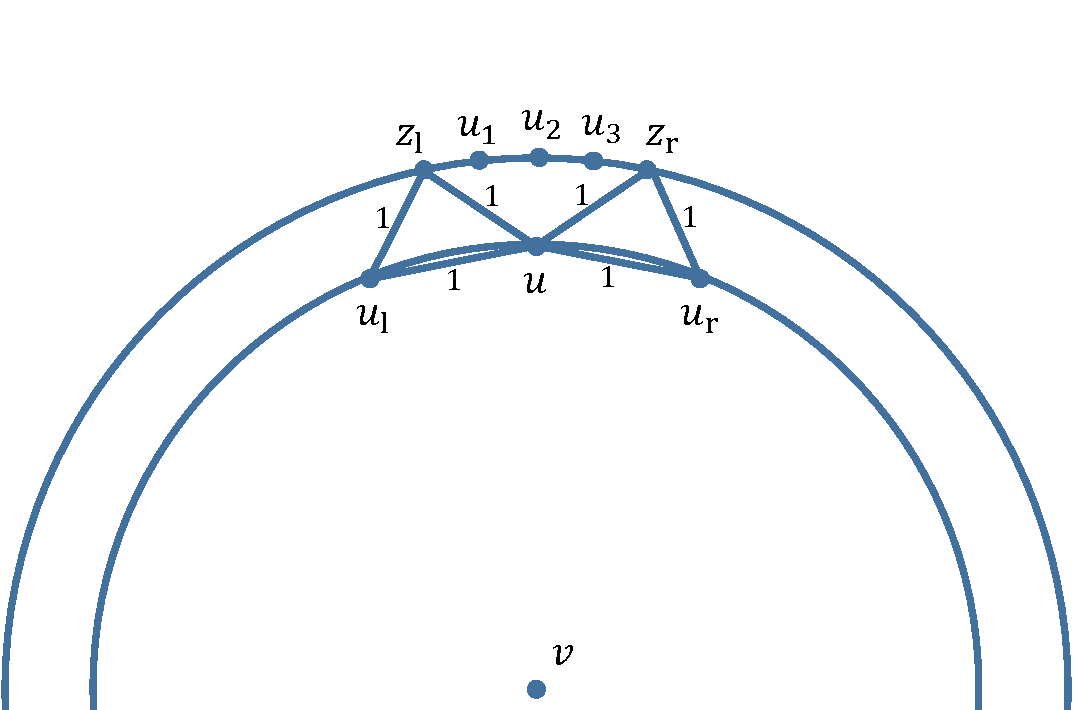
\includegraphics[width = 0.5 \textwidth]{trees.pdf}
    \caption{Threshold-based embedding of trees. The nodes $u_l, u$ and $u_r$ are at level $l$ while $u_1,u_2,u_3$ are at level $l+1$.}
    \label{fig:trees}
\end{figure}


For the lower bound on $C$, we have to guarantee that an embedding exists. For this, we provide the following construction (see Figure~\ref{fig:trees} for an illustration).
(Below we assume that the curvature is large enough for our construction to work, then we estimate the required curvature.)
First, we take the node $v$ and consider a circle of radius 1 around this node. 
We spread $b + 1$ neighbors uniformly around this node. For our construction to work, we need all distances between these nodes to be larger than 1.
Now, at some step of the algorithm, assume that we have all nodes at level $l$ placed at some circle centered at $v$ and all distances between the nodes at level $l$ are larger than 1. Our aim is then to find positions for all nodes at level $l + 1$.

Let us take any node at $l$-th level. Consider two points $u_l$ and $u_r$ on the same circle at distance 1 from the node $u$ to the left and to the right, respectively.
Let $u,u_l,z_l$ and $u,u_r,z_r$ form equilateral triangles (with sides equal to 1). Then we let the points at $l+1$-th level to be spread on the circle centred at $v$ and passing through $z_l$ and $z_r$. The children of $u$ ($u_1, \ldots, u_{b}$) will be placed on the circular arc between $z_l$ and $z_r$. As usual, we want $u_i$ and $u_{i+1}$ to be at distance at least 1 from each other. Moreover, they have to be at distance at least 1 from children of other nodes. Also, note that placing $u_1, \ldots, u_{b}$ between $z_l$ and $z_r$ guarantees that these nodes are closer than 1 to their parent node $u$ but at the same time at a distance larger than 1 from all other nodes at $l$-th level. Also, all points at $l$-th level are far enough from points at $l+2$-th level. 

It remains to find a maximum curvature such that the required conditions are satisfied. Let $r$ and $r'$ be radii of circles at $l$-th and $l+1$-th levels and let $2\alpha = \angle u_l v u$. We know (the law of cosines and $\cos 2\alpha = 1 - 2\sin^2 \alpha$) that
\begin{equation}\label{eq:1}
\cosh \frac{1}{R} = 1 + 2 \sinh \frac{r}{R} \sin^2 \alpha \,.
\end{equation}
So the only condition we need for the whole procedure to work is that we have enough space on the circular arc for placing $b$ nodes there:
\[
\cosh \frac{1}{R} \le 1 + 2 \sinh \frac{r'}{R} \sin^2 \frac{\alpha}{b} \,.
\]
We note that $\sin^2 \frac{\alpha}{b} \ge \frac{\sin^2 \alpha}{b^2}$ for all $b \ge 1$. Therefore, it is sufficient to have
\begin{equation}\label{eq:2}
\cosh \frac{1}{R} \le 1 + 2 \sinh \frac{r'}{R} \cdot \frac{\sin^2 \alpha}{b^2} \,.
\end{equation}
Combining \eqref{eq:1} and \eqref{eq:2}, we obtain:
\[
\sinh \frac{r'}{R} \ge b^2 \cdot \sinh \frac{r}{R}.
\]
To achieve this, it is sufficient to have: 
\[
\frac{r' - r}{R} \ge 2 \log b,
\]
\[
R \le \frac{r' - r}{2 \log b}.
\]
It remains to find the lower bound for $r' - r$ and it is easy to see that $r' - r$ decreases with $r$. Therefore, it is sufficient to consider only the second step of the construction procedure, when we move from the circle of radius 1 to the next one. In this case, $r = 1$ and 
\[
r' = 2 \, \mathrm{arccosh} \frac{\cosh 1}{\cosh 1/2}.
\]
So, we have 
\[
-C = \frac{1}{R^2} \le \left( \frac{2\,\log b}{2 \, \mathrm{arccosh} \frac{\cosh 1}{\cosh 1/2} - 1} \right)^2.
\]
\end{proof}

\subsection{Complete graph $K_n$}

\subsubsection{Ollivier curvature}  
For any two nodes $u$ and $v$, it follows from Example 1 in~\cite{jost2014ollivier} that $\kappa_{K_n}(v, u) = \frac{n-2}{n-1}$. Thus, $\kappa(K_n) = \frac{n-2}{n-1}$ and it tends to 1 as $n \to \infty$.

\subsubsection{Forman curvature} 
Simple computations yield:
$F(K_n) = 6 - 2n$, $\hat{F}(K_n) = n$, i.e., we get either highly positive or highly negative value.

\subsubsection{Average sectional curvature} It is easy to compute that
$\xi(K_n) = \frac{1}{8}$.

\subsubsection{Distortion-based curvature}

The following theorem analyzes $C_d^{dist}(K_n)$ if $d = n-2$. 

\begin{theorem}\label{thm:clique_distortion}
$C_{n-2}^{dist}(K_n) = \bigg\{-\infty,  4 \left(\arcsin \sqrt{\frac{n}{2(n-1)}}\right)^2\bigg\}$.
\end{theorem}

\begin{proof}
If $d = n-2$, then we are given a $(n-1)$-simplex, which can be embedded into $n-2$-dimensional spherical space. Indeed, the radius of circumscribed hypersphere for the $(n-1)$-simplex with side length $a$ is known to be $R = a\sqrt{\frac{n-1}{2n}}$. Since we want the \textit{spherical} distance between all points to be equal to one, we need to choose $a$ accordingly:
\[
\sin \frac{\alpha}{2} = \frac{a}{2R} \,\,\text{ for } \,\,\alpha = \frac{1}{R}.
\]
Here $\alpha$ corresponds to the angle giving the arc length 1, while the condition on $\sin \frac{\alpha}{2}$ relates $\alpha$ and $a$ since $\alpha$ is the angle in a triangle with side lengths $\alpha, R, R$.
This implies that
\[
2 R \arcsin \frac{a}{2R} = 1,
\]
and solving this equation for $a$ yields
%\[
%2 a\sqrt{\frac{n-1}{2n}} \arcsin \sqrt{\frac{n}{2(n-1)}} = 1,
%\]
\[
a  = \sqrt{\frac{2n}{(n-1)}}\frac{1}{2\arcsin \sqrt{\frac{n}{2(n-1)}}}.
\]
%\textbf{[I remember that it took me some time to properly follow this argument in the previous versions. Now I again have to spend some time to understand this. Could we maybe add some additional explanation?]}
Plugging this back into the formula for the radius $R$ we obtain
\[
R = \frac{1}{2\arcsin \sqrt{\frac{n}{2(n-1)}}},
\]
so that we have
\[
C_{n-2}^{dist}(K_n) = 4 \left(\arcsin \sqrt{\frac{n}{2(n-1)}}\right)^2\,.
\]

Finally, let us show that if $c \to -\infty$, then optimal distortion $D_{opt}(K_n) \to 0$. This result follows from the fact that $D_{opt}(S_n) \to 0$, because to embed a clique, it is sufficient to embed a star on $n+1$ node with edge lengths 1/2 and then remove the central node. 
\end{proof}


\subsubsection{Threshold-based curvature} 
$C_d^{thr}(K_n) = \R$, since we can embed any complete graph perfectly by mapping all nodes to one point. 

\subsection{Cycle graph $C_n$} 

We consider a cycle $C_n$ with $n \ge 4$.

\subsubsection{Ollivier curvature}  
Let $v \sim u$ be two neighbors. Then it is easy to see that $W_1^G(m_u,m_v) = 1$ and hence $\kappa_G(u,v) = 0$. Thus, $\kappa(C_n) = 0$.

\subsubsection{Forman curvature} 

Similarly, it is easy to see that $F(C_n) = \hat F(C_n) = 0$.

\subsubsection{Average sectional curvature} If $n$ is even, then $\xi_{C_n}(v;b,c;a) = 0$ for all points except the one diametrically opposite to $v$ for which we have $\xi_{C_n}(v;b,c;a) = 1$. If $n$ is odd, then for two points we have $\xi_{C_n}(v;b,c;a) = \frac{n}{2(n-1)}$. As a result, $\xi(C_n) = \frac{1}{n-3}$ for even $n$ and $\xi(C_n) = \frac{n}{(n-1)(n-3)}$ for odd $n$.

\subsubsection{Distortion-based curvature} 

%\begin{proposition}\label{prop:cycle_distortion}
%$C_d^{dist}(C_n) = \left(\frac{2\pi}{n}\right)^2$.
%\end{proposition}
Here we have that
%\begin{equation}\label{eq:cycle_distortion}
$	C_d^{dist}(C_n) = \left(\frac{2\pi}{n}\right)^2.$
%\end{equation}
Indeed, if we consider any three consequent nodes, then the middle one should lie on the geodetic between the other two. So, they all lie on a great circle (of length $n$) from which the result follows.

\subsubsection{Threshold-based curvature} 
It is easy to see that $C_d^{thr}(C_n) = (-\infty, C)$ with some $C>0$, which decreases with $n$ and increases with $d$. 
A simple lower bound for $C$ is $C \ge \left(\frac{4\pi}{n}\right)^2$, since for such curvature we can embed all nodes into a great circle with distances 1/2 between the closest ones. 


\subsection{Complete bipartite graph $K_{l,m}$}

W.l.o.g. we assume that $l \ge m \ge 2$ (the remaining cases are stars and are already considered). 

\subsubsection{Ollivier curvature}  
We prove the following lemma.

\begin{lemma}\label{lem:bipartite_ollivier}
$\kappa(K_{l,m}) = 0$.
\end{lemma}

\begin{proof}
Denote the node sets in $K_{l,m}$ by $U := \{u_1, \dots, u_l\}$ and $V := \{v_1, \dots, v_m\}$. We will prove that for any edge $(u, v)$, $W_1^{K_{l,m}}(m_{u},m_{v}) = 1$, which then implies that $\kappa(K_{l,m}) = 0$. For this we use the dual representation for the Wasserstein distance, see~\cite{ollivier2009ricci} for more details. This states that on the one hand
\[
	W^{G}_1(m_u,m_v) = \inf_{\rho} \sum_{v^\prime \sim v} \sum_{u^\prime \sim u} d_G(v^\prime, u^\prime) \rho(v^\prime, u^\prime),
\]
where the infimum is taken over all joint probability measures on the product of the neighborhoods of $v$ and $u$, while on the other hand
\[
	W^{G}_1(m_u,m_v) = \sup_{f} \left( \frac{1}{\mathrm{deg}(v) }\sum_{v^\prime \sim v} f(v^\prime) - \frac{1}{\mathrm{deg}(u) }\sum_{u^\prime \sim u} f(u^\prime)\right),
\]
where the supremum is taken over all $1$-Lipschitz functions, i.e., $|f(u) - f(v)| \le d_G(u,v)$.

Note that for any $u \in U, v \in V$ the joint neighborhood is $V \times U$. First we establish an upper bound by considering the product joint probability density on $V \times U$
$
	\rho(x,y) =	\frac{1}{m l}.
$
It then follows that
\[
	W_1^{K_{l,m}}(m_{u},m_{v}) \le \sum_{i = 1}^m \sum_{j = 1}^l d_G(v_i, u_j) \rho(v_i, u_j)
	= 1.
\]
For the lower bound, we define the function
\[
	f(z) = \begin{cases}
		2 &\mbox{if } z \in V,\\
		1 &\mbox{if } z \in U.
	\end{cases}
\]
Observe that if $u \in U$ and $v \in V$ then $|f(u) - f(v)| = 1 = d_G(u,v)$. On the other hand, if $u, u^\prime \in U$ then $|f(u) - f(u^\prime)| = 0 \le 2 = d_G(u,u^\prime)$ and similar for $v, v^\prime \in V$. Thus we conclude that $f$ is 1-Lipschitz. It now follows that
\[
	W_1^{K_{l,m}}(m_u,m_v) \ge \frac{1}{m} \sum_{i = 1}^m f(v_i) - \frac{1}{l} \sum_{j = 1}^l f(u_j) = 1,
\]
which completes the proof.
\end{proof}

\subsubsection{Forman curvature} 
It is easy to see that
$F(K_{l,m}) = \hat F(K_{l,m}) = 4 - l - m$. 

%\subsubsection{Approximate Ollivier curvature} 
%In is easy to derive from \eqref{eq:def_ollivier_ricci_approx} that $\kappa^*(K_{l,m}) = 0$. \textcolor{red}{[Which is probably significantly different from true Ollivier curvature.]}

\subsubsection{Average sectional curvature} 
The following lemma holds.

\begin{lemma}\label{lem:bipartite_heuristic}
$
\xi({K_{l,m}}) = \frac{-(l - m)^2 + m + l - 2}{(m+l-2)(l+m-3)}.
$
In particular, if $m = l$ we get $\xi({K_{l,m}}) = \frac{1}{2m - 3}$. 
\end{lemma}
This lemma implies that for balanced complete bipartite graphs $\xi({K_{l,m}})$ is positive, but tends to zero as the graph grows.

\begin{proof}
If $v$ and $a$ are in the same part of the bipartite graph, then $\xi_{K_{l,m}}(v;b,c;a) = 1$, otherwise $\xi_{K_{l,m}}(v;b,c;a) = -1$. Therefore, if $a$ belongs to the part of size $l$, sectional curvature is
$\xi_{K_{l,m}}(v;b,c) = \frac{l-m+1}{l+m-3}$, otherwise it is $\xi_{K_{l,m}}(v;b,c) = \frac{m-l+1}{l+m-3}$. As a result, by averaging over all triplets, we get

\begin{multline*}
\xi({K_{l,m}}) = \frac{1}{l \binom{m}{2} + m \binom{l}{2}} \left(l \binom{m}{2} \frac{l-m+1}{l+m-3} + m \binom{l}{2} \frac{m-l+1}{l+m-3}\right) \\
= \frac{-(l - m)^2 + m + l - 2}{(m+l-2)(l+m-3)}.
\end{multline*}
\end{proof}



\subsubsection{Distortion-based curvature} 

%Figure~\ref{fig:bipartite} (left) shows the empirical behavior of distortion depending on curvature. We observe that for all graphs optimal curvature (for the considered range) is between 2 and 2.5, where distortion has a drop. 
%The following proposition gives an intuition about why one could expect this. 
We prove the following simple proposition.

\begin{proposition}\label{prop:bipartite_distortion}
For any $d$, $C_d^{dist}(K_{2,2}) = \left(\frac{\pi}{2}\right)^2 \approx 2.47$ and $K_{2,2}$ is the only complete bipartite graph (with at least two nodes in each part) for which zero distortion is achievable.
\end{proposition}

\begin{proof}
Indeed, the result for $K_{2,2}$ follows from the corresponding result on cycle $C_4$. Moreover, if for $K_{l,m}$ we have $l \ge 3$ and $m \ge 2$, then for any two nodes in the part of size $l$ there are at least 2 different geodesics of length 2 between them. Therefore, all such pairs lie at opposite poles of the hypersphere, which is impossible since $l \ge 3$.
\end{proof}
%We also noticed in our experiments that very negative curvature can lead to even smaller distortion for bipartite graphs (see Table~\ref{tab:compare_distortion}).

%\subsubsection{Threshold-based curvature} Threshold-based embeddings to Euclidean spaces are well studied. In particular, it is know that for any graph $G(V,E)$ a perfect threshold embedding  exists for some $d \le |V|$~\cite{maehara1984space}. However, undirected bipartite graphs are hard to embed in Euclidean space: the bound $d = O(n)$ is known~\cite{maehara1984space}. We empirically observe that they are similarly hard to embed to both spherical and hyperbolic spaces, as shown in Figure~\ref{fig:bipartite} (right). Empirically, these graphs are insensitive to curvature (given that it is not too large).

\section{Conclusion}

We introduced a concept of global graph curvature motivated by the practical task of embedding graphs. This curvature depends on the loss function and space dimension. To get an intuition about how global graph curvature behaves, we theoretically analyzed it for several simple graphs. We compared the global graph curvature and several approximations based on well-known local graph curvatures and showed that they essentially differ. We demonstrated that dimensionality and the choice of a loss function fundamentally affect the global curvature and, in particular, when dimension is larger the optimal curvature usually becomes less negative. Our work shows that the problem of finding the rights space for graph embedding is interesting and non-trivial and we hope our results will encourage further research on global graph curvature.

% ---- Bibliography ----
%
% BibTeX users should specify bibliography style 'splncs04'.
% References will then be sorted and formatted in the correct style.
%
\bibliographystyle{splncs04}
\bibliography{curvature}
%

\newpage

\appendix

\section{Geometrical properties of spaces of constant curvature}\label{sec:properties}

In this section, we recall some useful equalities which will be used throughout the proofs.

We use notation $R$, where $R = \frac{1}{\sqrt{c}}$ in spherical space (corresponds to the radius of a sphere) and  $R = \frac{1}{\sqrt{-c}}$ in the hyperbolic case (can be considered as a scaling factor compared to the space of curvature~1).

\subsubsection{Law of cosines}

Let us consider a triangle with angles $A, B, C$ and the lengths of opposite sides $a, b, c$, respectively.

In Euclidean, space we have:
\[
c^2 = a^2 + b^2 - 2 \, a\, b \cos C\,.
\]

In spherical space, the first law of cosines is:
\[
\cos \frac{c}{R} =\cos \frac{a}{R} \cos \frac{b}{R} + \sin \frac{a}{R}\sin \frac{b}{R}\cos C \,,
\]
and the second law of cosines is:
\[
\cos C=-\cos A\cos B+\sin A\sin B\cos \frac{c}{R}\,.
\]

In hyperbolic space, we have 
\[
\cosh {\frac {c}{R}}= \cosh {\frac {a}{R}}\cosh {\frac {b}{R}}-\sinh {\frac {a}{R}}\sinh {\frac {b}{R}}\cos C \,.
\]

\paragraph{Equilateral triangle}

The following equalities follow from the corresponding laws of cosines, assuming that all sides (and angles) are equal.

For hyperbolic space:
\begin{equation}\label{eq:hyp_eq}
\cosh\frac{a}{2R} = \frac{1}{2\sin \frac{A}{2}}\,.
\end{equation}

For spherical space:
\begin{equation}\label{eq:sph_eq}
\cos{\frac{a}{R}} = \frac{\cos A}{1 - \cos A}.
\end{equation}

\subsubsection{Area and volume of hypersphere}

Let $S_d(r)$ and $V_d(r)$ denote area of a hypersphere and volume of a ball of radius $r$ in $d$-dimensional space. 

In euclidean space,
\[
S_d(r)= d \, C_{d} \, r^{d-1},
\]
\[
V_d(r)= C_{d} \, r^{d},
\]
where
\[
C_{d}={\frac  {\pi ^{{d/2}}}{\Gamma ({d \over 2}+1)}}.
\]

In spherical space, sphere of radius $r$ is isometric to Euclidean sphere of radius $R \sin \frac{r}{R}$. Therefore, the area is 
\[
S_d(r)= d \, C_{d} \, \left( R \sin \frac{r}{R} \right)^{d-1},
\]
\[
V_d(r)= d \, C_{d} \, R^d \int_{0}^{r} \left( \sin \frac{x}{R} \right)^{d-1} d x .
\]

Similarly, in hyperbolic space,
\[
S_d(r)= d \, C_{d} \, \left( R \sinh \frac{r}{R} \right)^{d-1},
\]
\[
V_d(r)= d \, C_{d} \, R^d \int_{0}^{r} \left( \sinh \frac{x}{R} \right)^{d-1} d x .
\]

\section{Proof of Theorem~\ref{thm:star_distortion}}\label{sec:proof:star_distortion}

First, let us analyze the lower bound on distortion. Recall that distortion of a graph is the average distortion over all pairs of nodes. Let $v$ be the central node and $v_1, \ldots, v_n$ ($n \ge 3$) be its neighbors. For any embedding $f$, we have
\begin{small}
\begin{multline*}
D(S_n) = \frac{1}{\binom{n+1}{2}} \left( \sum_{v_i} {|d(f(v),f(v_i)) - 1|} + \sum_{v_i \neq v_j} \frac{|d(f(v_i),f(v_j)) - 2|}{2} \right) \\
= \frac{1}{\binom{n+1}{2}} \sum_{1 \le i_1 < i_2 < i_3 \le n} \left(
\sum_{1\le j \le 3}  \frac{|d(f(v_{i_j}),f(v)) - 1|}{{n-1 \choose 2}} +
\sum_{1\le j < k\le 3}  \frac{|d(f(v_{i_j}),f(v_{i_k})) - 2|}{2(n-2)}   \right).
\end{multline*}
\end{small}

Let $D_{min}$ be the minimum value of the following weighted distortion of a star with 3 leaves:
\[
D_{min} = \min_{f} \sum_{1\le j \le 3}  \frac{|d(f(v_j),f(v)) - 1|}{(n-1)/4} +
\sum_{1\le j < k\le 3}  |d(f(v_j),f(v_k)) - 2|,
\]
then 
\begin{equation}\label{eq:D_min}
D(S_n) \ge \frac{{n\choose 3}}{2(n-2){n+1 \choose 2}} D_{min} = \frac{ (n-1)D_{min}}{6(n+1)}\,.
\end{equation}
Hence, it remains to find a lower bound on $D_{min}$, i.e., a lower bound for a weighted distortion of $S_3$ with central node $v$ and three leaves $v_1, v_2, v_3$.
If we consider three angles at the node $v$, then at least one of them is $\alpha \le 2 \pi / 3$, so we can get a lower bound by only considering this triangle, which is, w.l.o.g., formed by $v, v_1, v_2$.
\[
D_{min} \ge  |d(f(v_1),f(v_2)) - 2| + \frac{|d(f(v_1),f(v)) - 1| + |d(f(v_2),f(v)) - 1|}{(n-1)/2}.
\]

Denote $d(f(v_1),f(v)) = x = 1 + \varepsilon$, $d(f(v_2),f(v)) = y = 1 + \delta$, $d(f(v_1),f(v_2)) = z = 2 + \varepsilon + \delta - \varphi$ with some $\varepsilon, \delta$ and some $\varphi > 0$ (from triangle inequality). Assume that $|\varepsilon| < 1/2$ and $|\delta| < 1/2$ (otherwise the lower bound is trivial). Now we use the law of cosines to get a lower bound on $\varphi$.
We consider Euclidean and hyperbolic spaces separately and note that the bound obtained in Euclidean space also holds in spherical spaces (with any $c$).

In Euclidean space, using triangle inequality, we get  $\varphi = x + y - z > 0$. So, in Euclidean and spherical spaces $\varphi$ is bounded below by a constant.
%\[
%z^2 = x^2 + y^2 - 2 x y \cos \alpha, 
%\]
%so 
%\[
%(x+y)^2 - z^2 = 2 x y \lt{(\cos \alpha+1)}.
%\]
%As $\alpha < \pi$, we get
%$\varphi = x + y - z > 0$. 

In hyperbolic space the law of cosines gives 
(we denote $R = \frac{1}{\sqrt{-c}}$):
\[
\cosh \frac{z}{R} = \cosh \frac{x}{R} \cosh \frac{y}{R} - \sinh \frac{x}{R} \sinh \frac{y}{R} \cos \alpha,
\]
from which, using $\cosh(x+y) =\cosh x\cosh y+\sinh x\sinh y$, we get 
\[
\cosh \frac{x+y}{R} - \cosh \frac{z}{R} = \sinh \frac{x}{R} \sinh \frac{y}{R} (1 + \cos \alpha). %= \Omega\left(e^{(x+y)/R}\right).
\]
If $R \to \infty$, then, similarly to Euclidean case, we get $\varphi = x + y - z = \Omega(1)$. 

%\lt{[Replaced $\phi$ by $\varphi$]}
%\lt{[I do not quite follow the proof below, but the constant $\sqrt{c}$ is better and seems to hold. My idea of the proof was the following: let $x' = x/R, y' = y/R, z' = z/R, \varphi' = \varphi/R$. Then $x',y',z' \to \infty$ when $R \to 0$. Then $\sinh$ and $\cosh$ asymptotically behave as $e^{...}(1+o(1))/2$. Now, if I replace all $\sinh$ in the formula above, I derive that $e^{-\varphi'}$ cannot tend to 1, i.e., $\varphi'$ cannot tend to zero, i.e., $\varphi = \Omega(R)$]}
\iffalse
On the other hand, since $x+y - z = \varphi$, it follows from the mean value theorem that
\[
	\sinh \frac{x}{R} \sinh \frac{y}{R} (1 + \cos \alpha) = \frac{\varphi}{R^2} \sinh \frac{c}{R},
\]
for some $z \le c \le x + y$. Since $\sinh$ is monotonically increasing we deduce that
\[
	\frac{\varphi}{R^2} \ge (1+\cos \alpha) \frac{\sinh \frac{x}{R} \sinh \frac{y}{R}}{\sinh \frac{x+y}{R}}.
\]
Since the right hand side is bounded from below by a constant as $R \to 0$ it follows that $\varphi = \Omega(R^2)$ as $R \to 0$.
%}Otherwise,  have
%\[
%\cosh \frac{x+y}{R} - \cosh \frac{z}{R} = \Omega\left(e^{(x+y)/R}\right) = \Omega\left(e^{1/R}\right)
%\]
%and
%%$e^{\frac{x+y-z}{R}} - 1 = \Omega\left(e^{\frac{x+y-z}{R}}\right) = \Omega(1)$, so 
%$\varphi = x + y - z = \Omega(R)$. \ph{[I still do not follow this last step. Where does this conclusion come from and what are the asymptotics considered? It can't be $R \to \infty$ because we concluded that in that case it is bounded from below by a constant. So is it $R \to 0$?]}
\fi

On the other hand, if $R \to 0$, we get $\varphi = \Omega(R)$.
Note that $D_{min} \ge |z-2| + \frac{|x-1| + |y-1|}{(n-1)/2} =  |\varepsilon + \delta - \varphi| + \frac{|\varepsilon| + |\delta|}{(n-1)/2}$. This gives us a lower bound $D_{min} = \Omega(1/n)$ in spherical and Euclidean spaces and 
$D_{min} = \Omega(\min(R,1)/n) = \Omega\left(\frac{1}{n\max\left(\sqrt{-c},1\right)}\right)$ in hyperbolic space.
From this and \eqref{eq:D_min} the bound on $D(S_n)$ follows.
%\ph{$D_{min} = \Omega(\min(R^2,1)/n) = \Omega\left(\frac{1}{n\max\left(-c,1\right)}\right)$ in hyperbolic space}. \ph{Shouldn't this be $\min(R^2, 1/n)$?} From this and \eqref{eq:D_min} the required bound follows.

Now, let us get an upper bound on optimal distortion $D_{opt}(S_n)$. To do this, we explicitly construct an embedding with sufficiently low distortion $D(S_n)$.

Let $v$ be the central node, then we spread all other nodes uniformly on a 2-dimensional circle of radius $1$ centred at $v$. The smallest angle between two points is $2 \pi / n$. Therefore, from the law of cosines, the distance between leaves is at least $k$ with
\[
\cosh \frac{k}{R} = 1  + \left(1 -  \cos \frac{2 \pi}{n}\right)  \sinh^2 \frac{1}{R} \,.
\]

Note that for any two leaves $v_i$ and $v_j$ we have that $d(f(v_i), f(v_j)) \le 2$. In particular, the closer two leaves are, the greater the difference $2 - d(f(v_i), f(v_j))$ is. Hence, the distance between adjacent leaves is the worst case and thus $D_{opt}(S_n)$ can be upper bounded as
\begin{multline*}
D_{opt}(S_n) \le \frac{{n \choose 2}}{2{n+1\choose 2}} \left(2 - R\cdot \mathrm{arccosh}\left( \left(1 - \cos \frac{2 \pi}{n}\right)\sinh^2\frac{1}{R}  + 1 \right)\right) \\
= \frac{(n-1)}{2(n+1)} \left(2 - R\cdot \mathrm{arccosh}\left( \left(1 - \cos \frac{2 \pi}{n}\right)\sinh^2\frac{1}{R}  + 1 \right)\right)\,.
\end{multline*}
Note that $1 - \cos\frac{2\pi}{n} = \Theta\left(\frac{1}{n}\right)$ and $\sinh^2\left(\frac{1}{R}\right) = \Theta\left(e^{2/R}\right)$.
Then, the value $\textrm{arccosh}\left(\Theta\left(\frac{1}{n} e^{2/R}\right) + 1 \right)$ behaves as $\sqrt{2e^{2/R}/n}$ if $2/R \ll \log n$ and as $\frac{2}{R} - \log n$ if $2/R \gg \log n$.
Therefore, we get
\[
D_{opt}(S_n) = O\left( R \log n \right) = O\left( \frac{\log n}{\sqrt{-c}} \right).
\]



\section{Proof of Theorem~\ref{thm:star_threshold}}\label{app:proof:star_threshold}

Let us construct a perfect embedding of $S_n$ for $d = 2$
and estimate the required curvature.
Recall that in a perfect embedding all leaves have to be inside the ball of radius 1 around the central node $v$ and also the distance between any two leaves has to be larger than one. 
It is easy to see that if we managed to spread $n$ points inside the ball of radius 1 with distances more than 1 between them, then we can move each point along the radius up to distance 1 from $v$ preserving this property. Therefore, it is sufficient to spread all points on a hypersphere.

First, assume that $n > 6$. In this case we have to consider only hyperbolic space, since $n$ neighbors would not fit to a circle of radius 1 in neither spherical nor Euclidean spaces.
We will find the largest curvature $C$ which allows to have distance exactly 1 between the closest leaves. In this case we cannot embed $S_n$ in a space of curvature $C$, but can embed in a space of any smaller curvature. 
We use \eqref{eq:hyp_eq} (where $R = \frac{1}{\sqrt{-C}}$) and let $\alpha = \frac{2\pi}{n}$:
%\[
%\cosh{\frac{1}{k}} = \cosh^2{\frac{1}{k}} - \sinh^2{\frac{1}{k}}\cos\alpha.
%\]
%\[
%\cosh{\frac{1}{k}} = 1 +  (1- \cos\alpha) \sinh^2{\frac{1}{k}}.
%\]
%\[
%\cosh{\frac{1}{k}} = 1 +  2\sin^2 \frac{\alpha}{2} \sinh^2{\frac{1}{k}}.
%\]
%\[
%\frac{1}{2\sin^2 \frac{\alpha}{2}} = \frac{\sinh^2{\frac{1}{k}}}{\cosh{\frac{1}{k}} - 1}.
%\]
%\[
%\frac{1}{2\sin \frac{\alpha}{2}} = \frac{\sinh{\frac{1}{k}}}{\sqrt{2}\sqrt{\cosh{\frac{1}{k}} - 1}}.
%\]
\[
\cosh\frac{1}{2R} = \frac{1}{2\sin \frac{\alpha}{2}},
\]
\[
R = \frac{1}{2\,\textrm{arccosh}\frac{1}{2\sin \frac{\alpha}{2}}},
\]
\[
C = - \left(2\,\textrm{arccosh}\frac{1}{2\sin \frac{\alpha}{2}}\right)^2.
\]
Note that if $n$ is large, then $\sin \frac{\alpha}{2} = \sin\frac{\pi}{n-1} \sim \frac{\pi}{n-1}$. Then,  $\textrm{arccosh}\frac{1}{2\sin \frac{\alpha}{2}} \sim \textrm{arccosh}\frac{n-1}{2\pi} \sim \log n$, so we get $C \sim - 4 \log^2 n$. 

Now, let us consider $n \le 6$. Obviously, for $n = 6$ we have $C = 0$. 
%\textbf{[ I guess this is obvious because it is in Euclidean space. Maybe we should explain this a bit more.]}

If $n < 6$, then $C > 0$. 
In this case we consider a spherical space and use the corresponding law of cosines~\eqref{eq:sph_eq}:
\[
\cos{\frac{1}{R}} = \frac{\cos \alpha}{1 - \cos \alpha},
\]
\[
C = \left(\arccos \frac{\cos \alpha}{1 - \cos \alpha}\right)^2.
\]


\end{document}